\section{Experiments and Results}

\subsection{Training Setup}

All experiments were conducted in Google Colab Pro using a high-RAM GPU runtime. We used TensorFlow (Keras) and the Hugging Face Transformers library to build and train our models.

The dataset was split into:
\begin{itemize}
    \item \textbf{Training set:} 60\% (12,000 samples)
    \item \textbf{Validation set:} 20\% (4,000 samples)
    \item \textbf{Test set:} 20\% (4,000 samples)
\end{itemize}

This stratified split ensured balanced label distribution across all sets. Both models (DNN and CNN) were trained using the same configuration:

As mentioned earlier, both models were trained using the same configuration to ensure a fair comparison. The training setup included a \textbf{Binary Cross-Entropy} loss function, the \textbf{Adam} optimizer, a \textbf{batch size of 32}, and \textbf{early stopping} with a patience of 3 epochs (restoring the best weights). The maximum number of epochs was set to \textbf{10}. We used consistent tabular preprocessing and a frozen BERT text encoder across both models to isolate the effect of the tabular branch (DNN vs. CNN) in our comparison.

\subsection{DNN Results}

\textbf{Training Summary:}  
The DNN model trained for 6 epochs before early stopping. As shown in Figure~\ref{fig:dnn_acc_loss}, training accuracy steadily increased, reaching above 84\%, while validation accuracy peaked early around 66.5\% and then dropped, signaling overfitting. The training loss decreased sharply, while the validation loss climbed after epoch 2, confirming this behavior.

\begin{figure}[H]
    \centering
    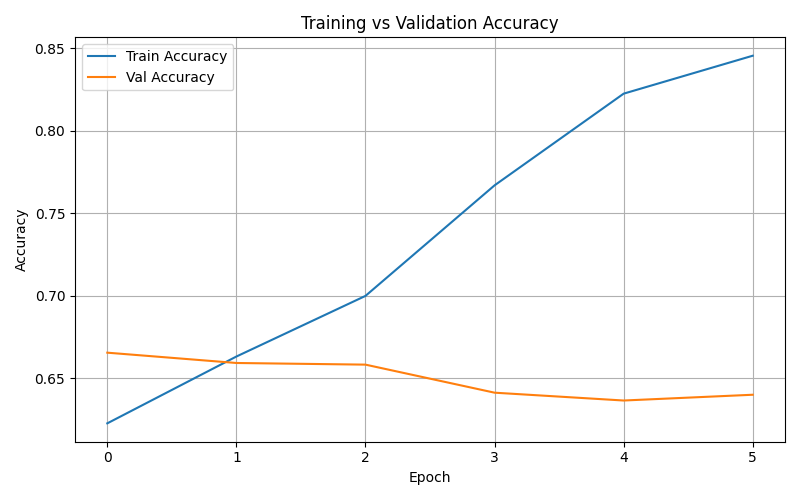
\includegraphics[width=0.47\linewidth]{figures/dnn_accuracy.png}
    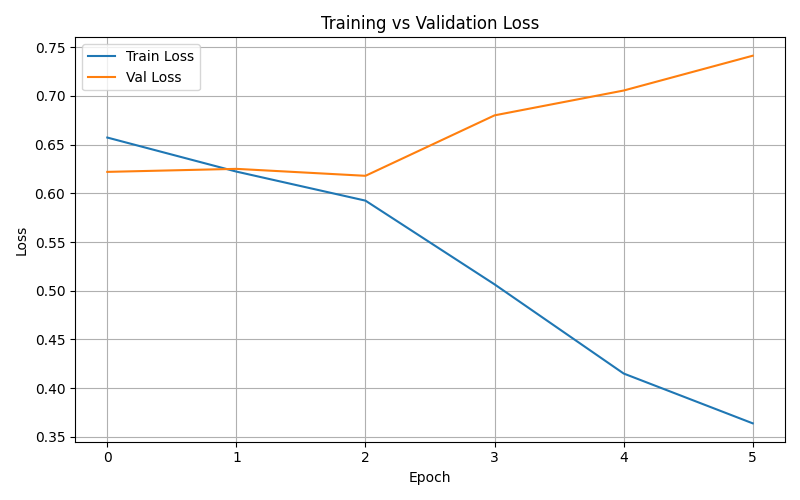
\includegraphics[width=0.47\linewidth]{figures/dnn_loss.png}
    \caption{DNN Training vs Validation Accuracy (left) and Loss (right)}
    \label{fig:dnn_acc_loss}
\end{figure}

\textbf{Evaluation Metrics:}  
On the 4,000-sample test set, the DNN achieved the following performance:

\begin{itemize}
    \item \textbf{Accuracy:} 64\%
    \item \textbf{Precision:} 0.68 (Class 1 – approved)
    \item \textbf{Recall:} 0.54 (Class 1)
    \item \textbf{F1-Score:} 0.60
    \item \textbf{ROC AUC:} 0.696
\end{itemize}

Figure~\ref{fig:dnn_conf_roc} illustrates the confusion matrix and ROC curve. The confusion matrix reveals that the model correctly rejects 1,487 non-eligible applicants but incorrectly approves 513 of them, posing a financial risk. More critically, it misses 916 eligible applicants (false negatives), reflecting a conservative bias that could lead to missed business opportunities. The ROC curve indicates a moderately strong classifier, with an AUC close to 0.70, suggesting decent but improvable discrimination between approved and rejected applicants.


\begin{figure}[H]
    \centering
    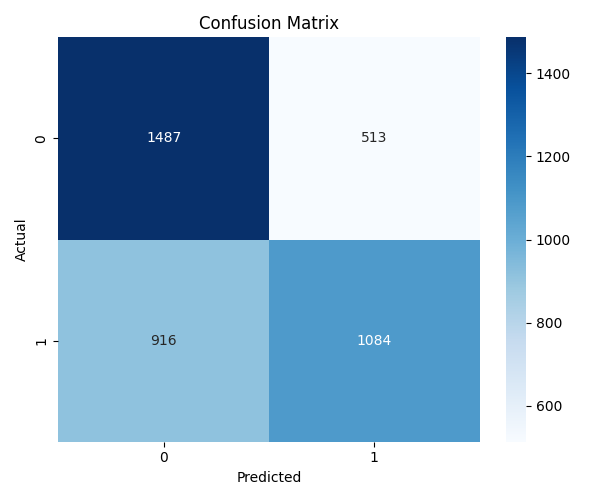
\includegraphics[width=0.47\linewidth]{figures/dnn_confusion_matrix.png}
    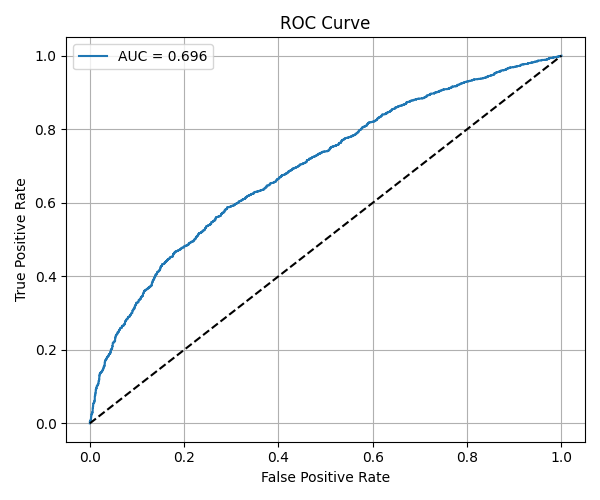
\includegraphics[width=0.47\linewidth]{figures/dnn_roc_curve.png}
    \caption{DNN Confusion Matrix (left) and ROC Curve (right)}
    \label{fig:dnn_conf_roc}
\end{figure}
\newpage
\textbf{SHAP Explainability:}  
We applied SHAP to gain insight into what the DNN was focusing on when making decisions.

Figure~\ref{fig:dnn_shap_global} presents the global feature importance from SHAP applied over 300 test samples. Key influential features included:
\begin{itemize}
    \item \texttt{home\_ownership\_MORTGAGE} (Home ownership = MORTGAGE) and \texttt{open\_acc} (Number of open credit lines) had a positive influence on approval.
    \item \texttt{fico\_range\_high} (Estimated credit score) and \texttt{annual\_inc} (Annual income) were related to credit quality.
    \item Categorical features like \texttt{verification\_status} (Income verification status) also showed consistent impact.
\end{itemize}

\begin{figure}[H]
    \centering
    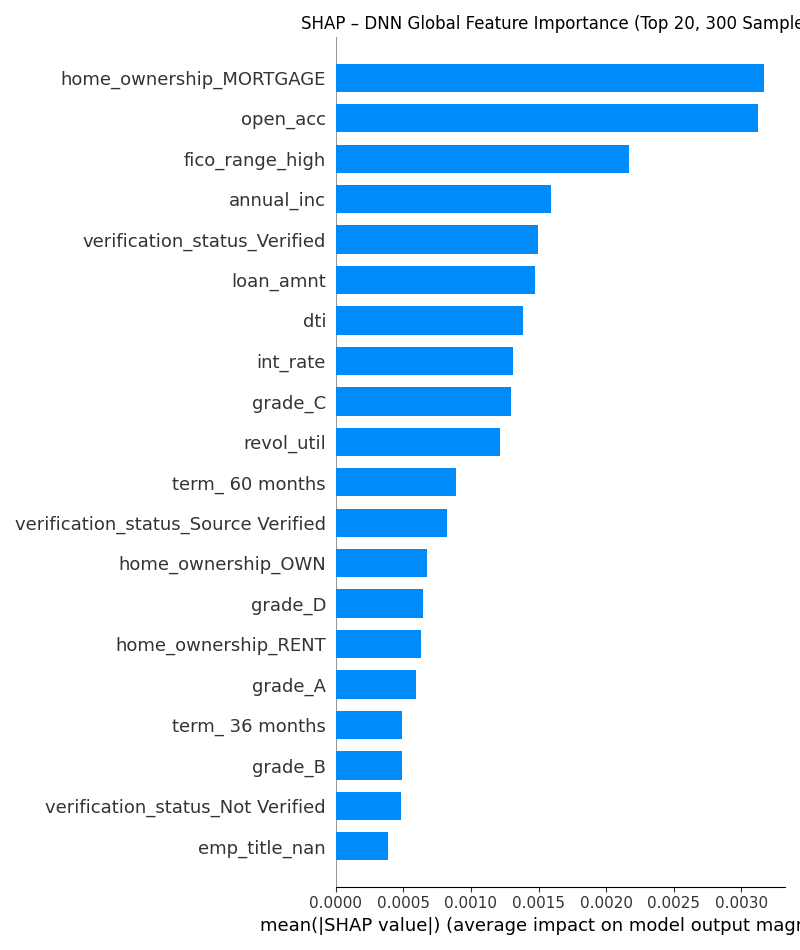
\includegraphics[width=0.85\linewidth]{figures/shap_dnn_global.png}
    \caption{DNN Global SHAP Values (Top 20 Features)}
    \label{fig:dnn_shap_global}
\end{figure}

Figure~\ref{fig:dnn_shap_local} shows a force plot for one specific prediction. In this sample, high \texttt{fico\_range\_high} (Estimated credit score) and \texttt{annual\_inc} (Annual income) increased the approval probability, while low \texttt{open\_acc} (Number of open credit lines) and renting status (\texttt{home\_ownership\_RENT}) pulled the prediction down. SHAP reveals how the model balances competing signals in a real example.

\begin{figure}[H]
    \centering
    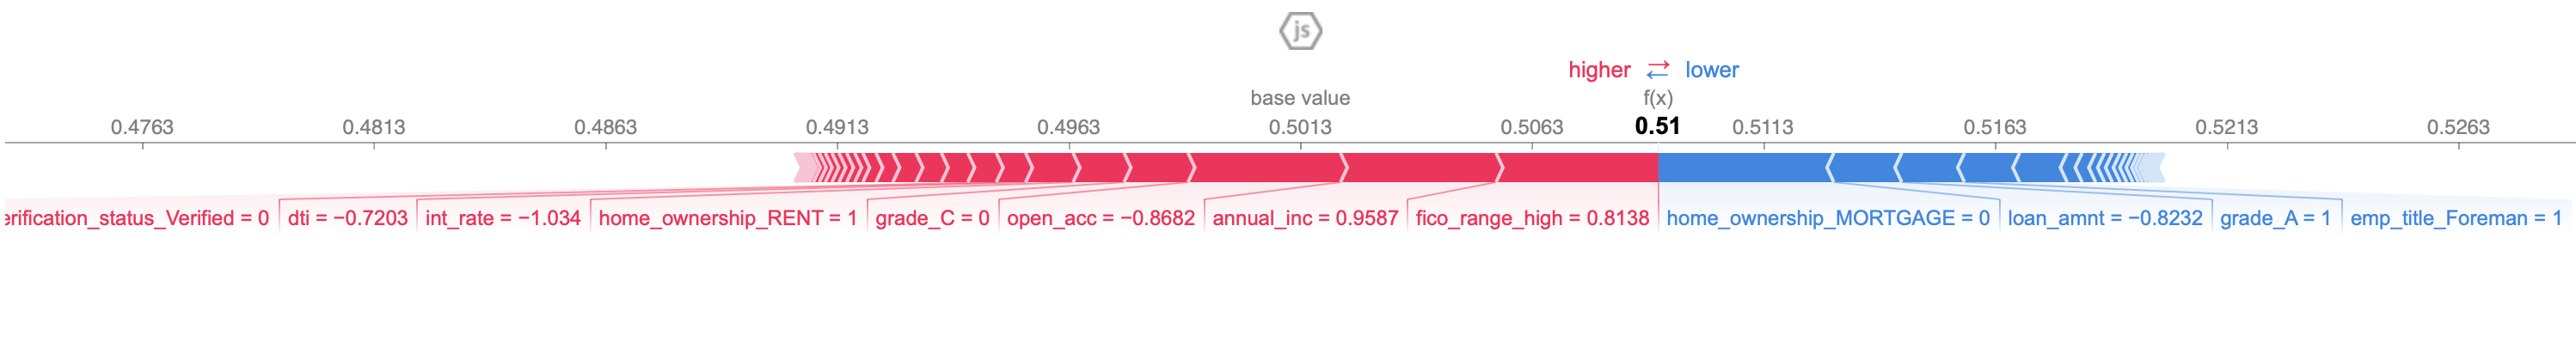
\includegraphics[width=0.95\linewidth]{figures/shap_dnn_force.png}
    \caption{DNN SHAP Force Plot for a Single Test Sample}
    \label{fig:dnn_shap_local}
\end{figure}

\textbf{Observations:}
\begin{itemize}
    \item The DNN showed strong training performance but suffered from mild overfitting on validation.
    \item SHAP provided clear interpretability for both global and local predictions.
    \item The model successfully leveraged both financial and categorical features to guide predictions.
\end{itemize}

\newpage
\subsection{CNN Results}

\textbf{Training Summary:}  
The CNN model trained for 5 full epochs before early stopping. Figure~\ref{fig:cnn_acc_loss} shows that both training and validation accuracy remained relatively stable. Validation accuracy peaked slightly at epoch 3, while training accuracy increased modestly. As seen in the loss plot (right), the validation loss hovered around 0.619 throughout training, suggesting minimal overfitting and a stable learning process.

\begin{figure}[H]
    \centering
    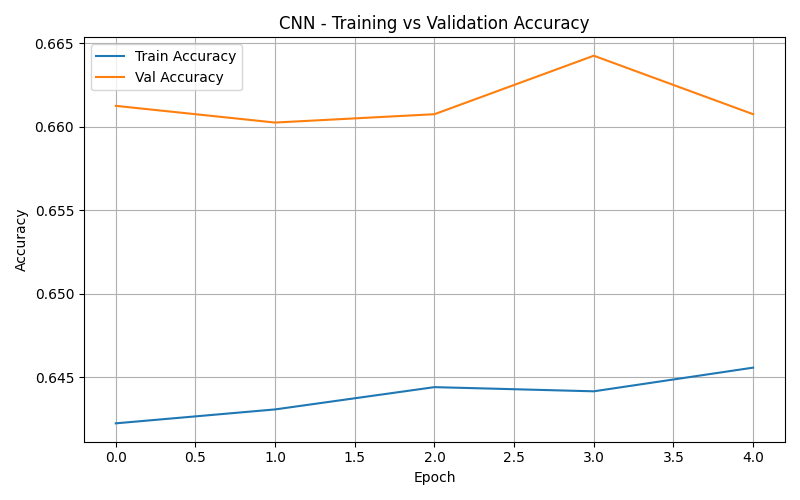
\includegraphics[width=0.47\linewidth]{figures/cnn_accuracy.png}
    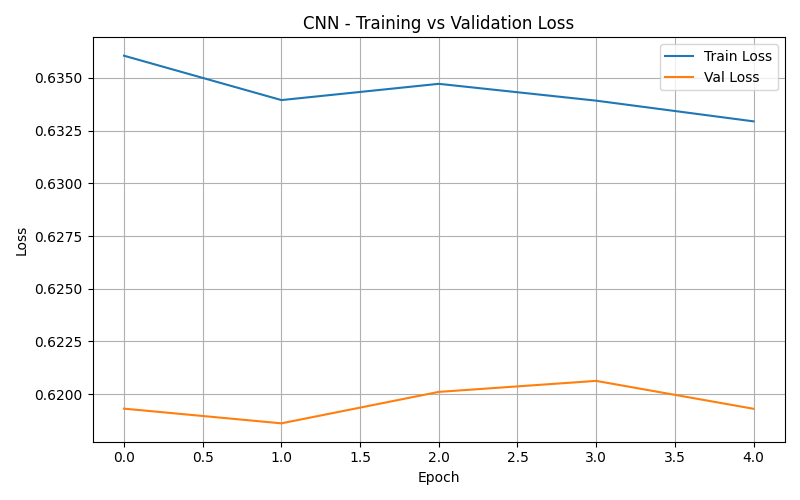
\includegraphics[width=0.47\linewidth]{figures/cnn_loss.png}
    \caption{CNN Training vs Validation Accuracy (left) and Loss (right)}
    \label{fig:cnn_acc_loss}
\end{figure}

\textbf{Evaluation Metrics:}  
The CNN achieved the following on the 4,000-sample test set:

\begin{itemize}
    \item \textbf{Accuracy:} 64\%
    \item \textbf{Precision:} 0.65 (Class 1 – approved)
    \item \textbf{Recall:} 0.60 (Class 1)
    \item \textbf{F1-Score:} 0.62
    \item \textbf{ROC AUC:} 0.692
\end{itemize}

Figure~\ref{fig:cnn_conf_roc} shows that the CNN was slightly more recall-focused than the DNN. This is evident from the confusion matrix, where it detected more true positives (1,200), though at the cost of more false positives. The ROC curve also confirms reasonable class separation, consistent with AUC performance.

\begin{figure}[H]
    \centering
    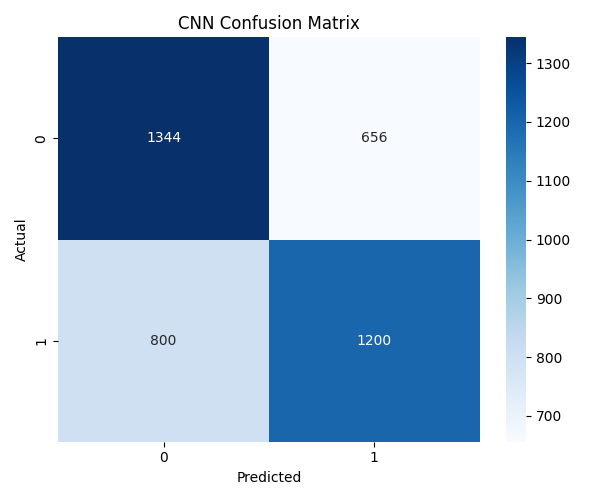
\includegraphics[width=0.47\linewidth]{figures/cnn_confusion_matrix.png}
    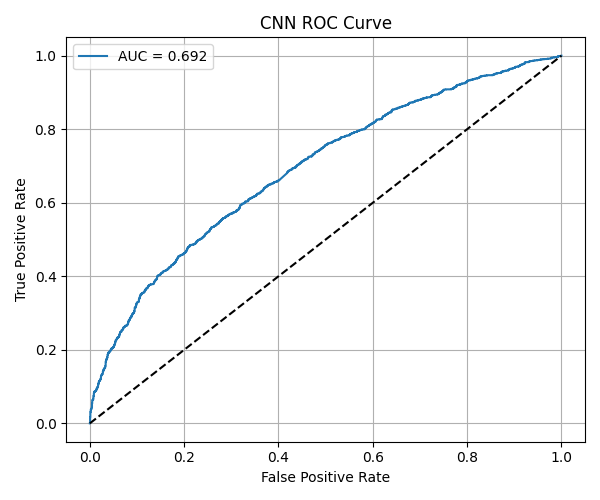
\includegraphics[width=0.47\linewidth]{figures/cnn_roc_curve.png}
    \caption{CNN Confusion Matrix (left) and ROC Curve (right)}
    \label{fig:cnn_conf_roc}
\end{figure}

\textbf{SHAP Explainability:}  
To understand feature contributions, we applied SHAP to the CNN model’s predictions.

Figure~\ref{fig:cnn_shap_global} presents the global SHAP values. The CNN relied more heavily on a few core features:
\begin{itemize}
    \item \texttt{fico\_range\_high} (Credit score estimate) and \texttt{open\_acc} (Number of open credit lines) were the top predictors.
    \item Other contributors included \texttt{dti} (Debt-to-income ratio), \texttt{grade\_B} (Loan grade = B), and \texttt{revol\_util} (Revolving credit utilization rate).
    \item Compared to the DNN, fewer categorical variables had strong influence.
\end{itemize}

\begin{figure}[H]
    \centering
    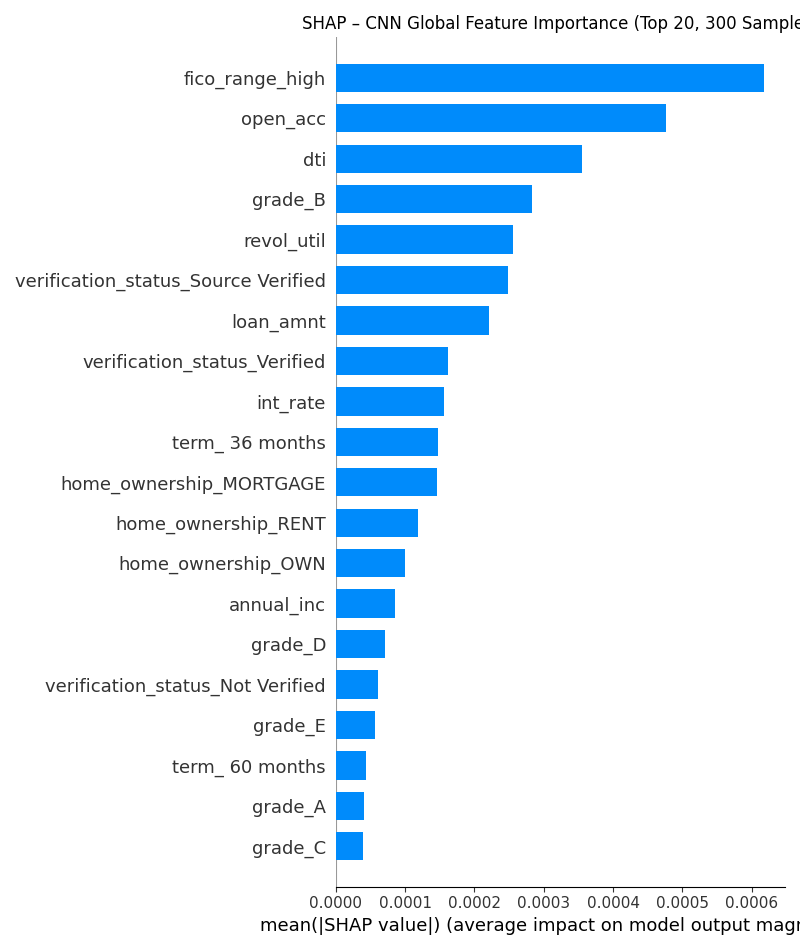
\includegraphics[width=0.85\linewidth]{figures/shap_cnn_bar.png}
    \caption{CNN Global SHAP Values (Top 20 Features)}
    \label{fig:cnn_shap_global}
\end{figure}

The force plot in Figure~\ref{fig:cnn_shap_local} explains a single prediction. High \texttt{fico\_range\_high} (credit score estimate), a positive \texttt{emp\_title\_Foreman} (job title = Foreman), and an unverified \texttt{verification\_status} pushed the score upward, while low \texttt{open\_acc} (number of open credit lines) and high \texttt{dti} (debt-to-income ratio) pulled it down. This demonstrates how the CNN focuses on fewer, sharper indicators.

\begin{figure}[H]
    \centering
    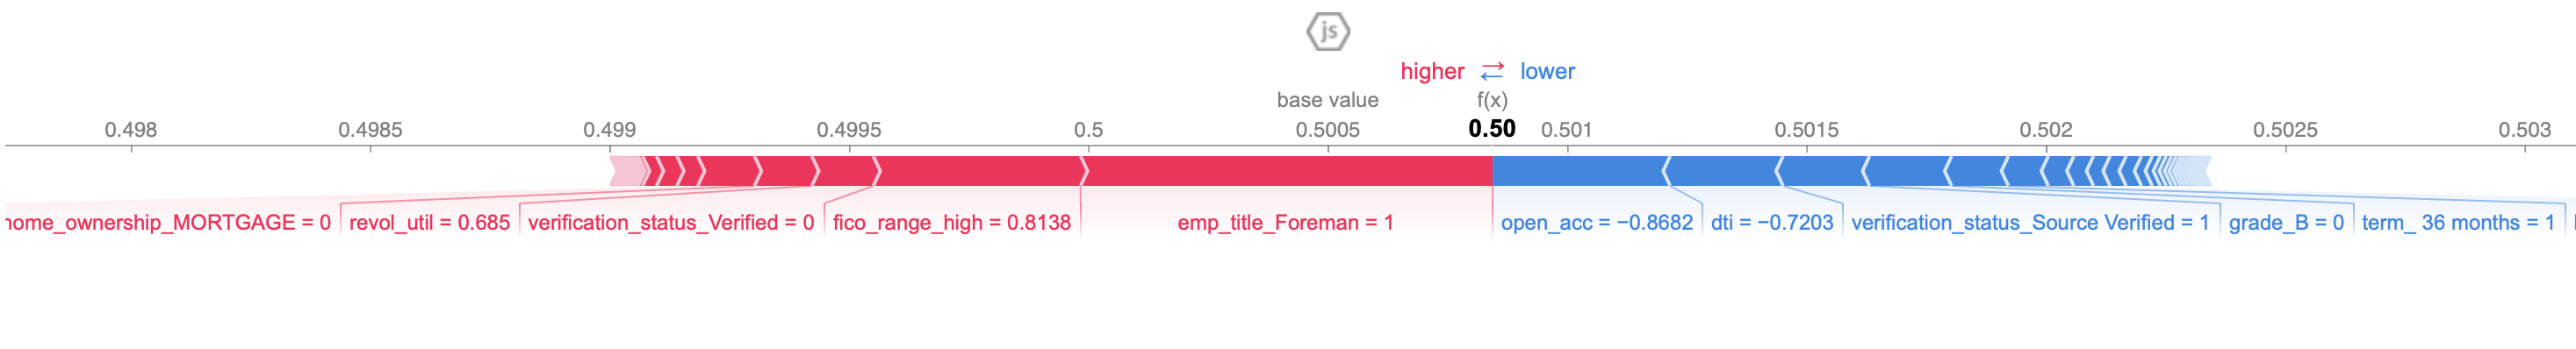
\includegraphics[width=0.95\linewidth]{figures/shap_cnn_force.png}
    \caption{CNN SHAP Force Plot for a Single Test Sample}
    \label{fig:cnn_shap_local}
\end{figure}

\vspace{1em}
\newpage

\textbf{Observations:}
\begin{itemize}
    \item The CNN model matched the DNN in performance, despite being more lightweight (58K vs. 465K parameters).
    \item SHAP interpretation suggests the CNN learned to rely on fewer but more dominant features.
    \item Higher recall and F1-score make it valuable for reducing false negatives in sensitive use cases like loan approvals.
    
\end{itemize}
\vspace{-1em}   % Negative space pulls things upward

\subsection{Model Comparison and Analysis}

To summarize the differences and trade-offs between the DNN and CNN architectures, we compared them across performance, interpretability, and complexity dimensions.

\textbf{Performance Metrics:}  
Both models achieved identical accuracy (64\%) on the 4,000-sample test set. However, the CNN achieved slightly higher \textbf{recall} (0.60 vs. 0.54) and \textbf{F1-score} (0.62 vs. 0.60), making it more effective at capturing approved loans. On the other hand, the DNN had slightly higher \textbf{precision} (0.68 vs. 0.65), suggesting it was more conservative in predicting approvals.

\textbf{ROC-AUC Comparison:}  
Figure~\ref{fig:roc_comparison} shows that both models had similar AUC scores:  
DNN = 0.696, CNN = 0.692. The nearly overlapping ROC curves confirm that both models had comparable class separation abilities.

\begin{figure}[htbp]
    \centering
    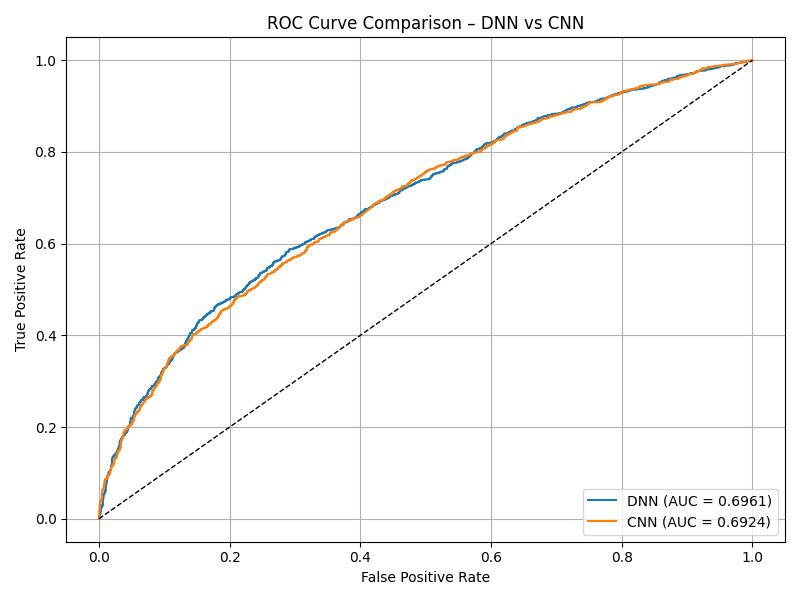
\includegraphics[width=0.75\linewidth]{figures/roc_comparison_dnn_vs_cnn.png}
    \caption{ROC Curve Comparison – DNN vs CNN}
    \label{fig:roc_comparison}
\end{figure}

\textbf{Model Complexity:}  
The DNN used \textbf{464,929 trainable parameters}, while the CNN operated with only \textbf{58,817}. This makes the CNN more efficient and suitable for environments with limited computational resources. Despite the drastic reduction in model size, the CNN matched the DNN’s accuracy and even surpassed it in recall.

\vspace{0.5em}
\vspace{1cm}
\textbf{Training Time Estimates:}
\begin{itemize}
    \item \textbf{DNN:} ~353 seconds (6 epochs)
    \item \textbf{CNN:} ~330 seconds (5 epochs)
\end{itemize}
Although slightly faster, CNN's time savings were marginal due to similar architecture fusion and BERT usage.

\textbf{Explainability Comparison:}  
SHAP analysis revealed clear contrasts in how the models made decisions:
\begin{itemize}
    \item The \textbf{DNN} produced a more distributed feature attribution, considering a broader range of numerical and categorical variables.
    \item The \textbf{CNN}, however, focused more narrowly on a handful of strong predictors such as \texttt{fico\_range\_high}, \texttt{open\_acc}, and \texttt{dti}.
\end{itemize}
This focused behavior aligns with CNN’s inductive bias of extracting localized patterns, even when applied to tabular data.

\textbf{Interpretation:}  
The DNN may be preferable when nuanced feature contributions are needed, especially for stakeholder explainability. The CNN’s higher recall and simplicity make it compelling for real-time or edge deployment scenarios.

\textbf{Overall Insight:}  
While both models performed similarly, the CNN’s lightweight nature, slightly better recall, and sharp SHAP explanations position it as a promising alternative. However, the DNN’s broader feature awareness and interpretability remain valuable in high-stakes decisions.